%% ----------------------------------------------------------------
%% Introduction.tex
%% ---------------------------------------------------------------- 
\chapter{Background Research} \label{Chapter:Background Research}
% PR-Anurag - COMPLETED 1    
\section{Wireless Telemetry Data} \label{section:WirelessTelemetryResearch}

The initial component to this project is the retrieval of wireless telemetry data. Telemetry is the automatic measurement and wireless transmission of data from a remote or inaccessible source for monitoring. The telemetry data source for this project is an 802.11ax Wi-Fi router acting as a Wireless Access Point. 

\subsection{ASUS ROG Rapture GT-AX11000 Router}

The ASUS ROG GT-AX11000 (provided by InterDigital) is a Tri-band 10 Gigabit Wi-Fi router with a quad-core CPU. It supports 2.4GHz, 5GHz-1 and 5GHz-2 bands with a combination of OFDMA and MU-MIMO technology to provide greater network capacity and efficiency. The use of Orthogonal Frequency Division Multiple Access (OFDMA) allows for one channel to transmit data to several devices at the same time (more on this later) \cite{OFDMA}. 

\subsection{ASUS Web GUI}

Out the box, ASUS provides an intuitive web Graphical User Interface (The ROG Gaming Centre) that acts as the main hub for total network control, with need-to-know information such as connected device status, server ping values, real-time network traffic and much more. Built into the web GUI are a multitude of features and operational settings, some of which will now be further explored. 

\subsubsection{Dash Board}

The Dash Board, as shown in Figure \ref{fig_ASUSwebGUI}, allows the network administrator to monitor real-time traffic metrics for the networking environment and analyse the real-time network ping and ping deviation.


\begin{figure} [ht]
    \centering
    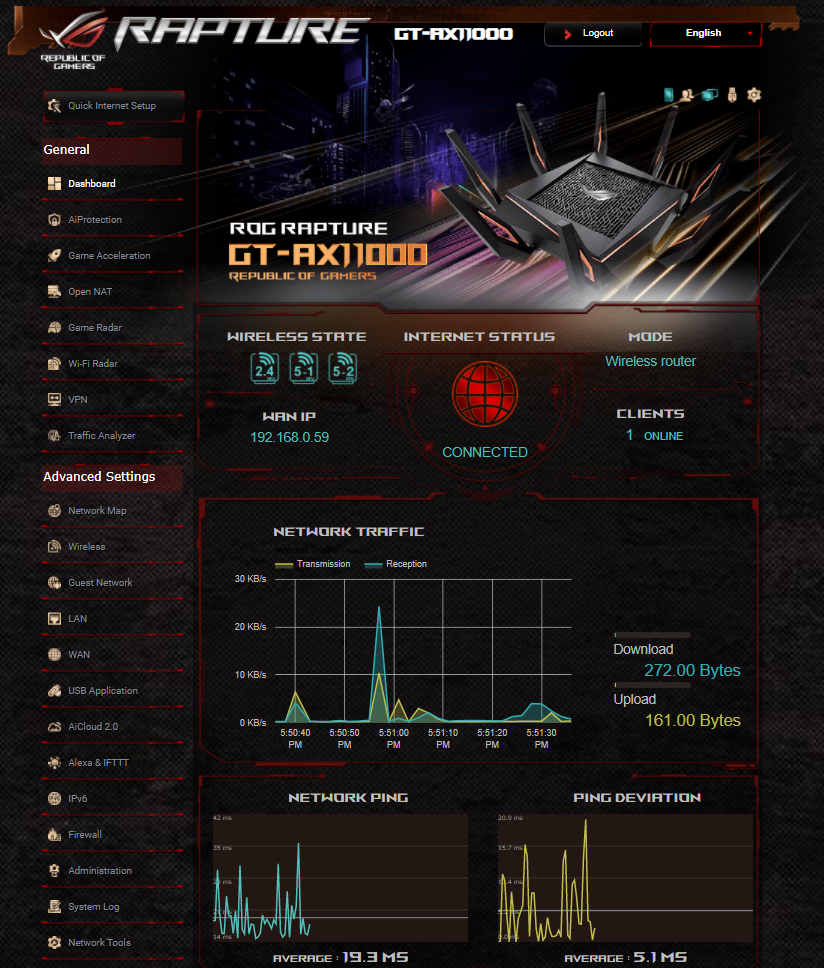
\includegraphics[width=1\linewidth]{pages/Chapter2/Chapter 2 images/ASUSwebGUI.PNG}
    \caption{ASUS ROG Gaming Centre.}
    \label{fig_ASUSwebGUI}
\end{figure}

\subsubsection{WiFi Radar}

WiFi Radar is an advanced analysis tool for the wireless network, it delves deep into the wireless channels and packet data intended for the purposes of troubleshooting. This feature permits the user to perform a Wi-Fi site survey in order to gather information on all nearby wireless access points. The site survey displays the signal strength, signal-to-noise ration (SNR), maximum physical rate, bandwidth and channel information. 




\begin{figure} [ht]
    \centering
    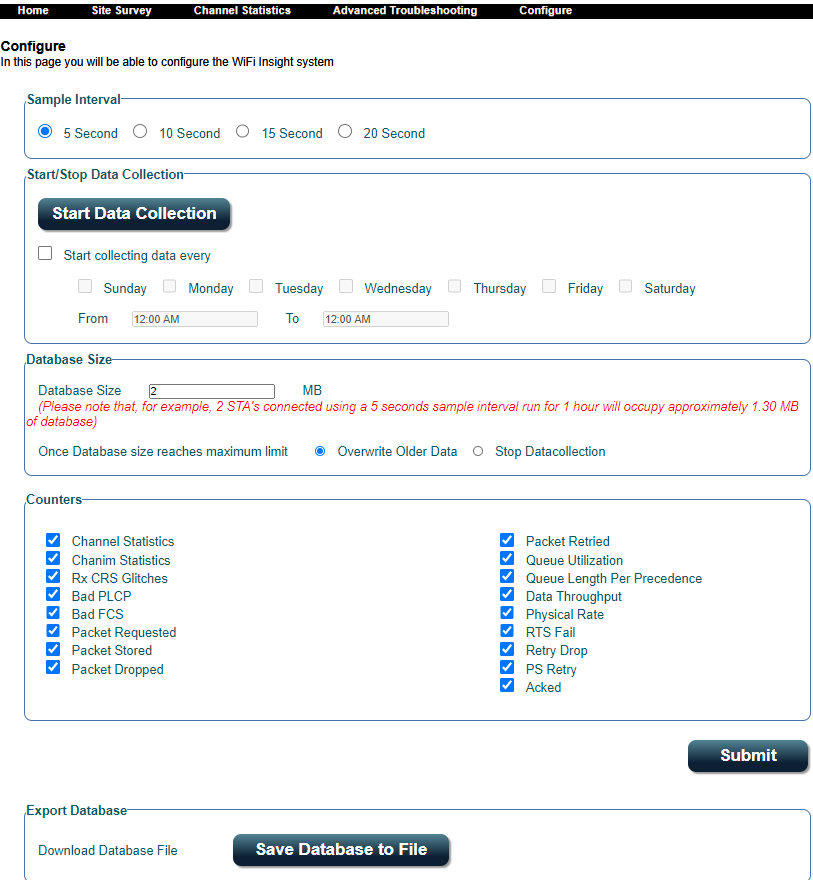
\includegraphics[width=1\linewidth]{pages/Chapter2/Chapter 2 images/WiFiRadarSetting.PNG}
    \caption{Advanced Troubleshooting Page on ASUS Web GUI.}
    \label{fig_WiFiRadar}
\end{figure}

Additionally, the Advanced Troubleshooting feature provides a telemetry data collection option, as shown in figure \ref{fig_WiFiRadar}, which produces a database with all technical data about the various advanced Wi-Fi parameters. This WiFi Radar component records data and generates a .DB file which is size configurable. This means that the user can define a maximum size that the database can reach after which it will either overwrite the older data or just stop data collection altogether. Also, the sample interval is configurable with settings to have data recorded every 5, 10, 15 or 20 seconds. Moreover, ASUS state that collecting data using a 5 second sample interval and with 2 STA’s (Stations) for 1 hour will approximately occupy 1.3MB of database, with new datasets being appended to the existing file. 

Appendix B Section \ref{ASUSEmail} shows an email correspondence with the ASUS customer service team asking to provide additional documentation for purposes of research and project work. Since ASUS could not provide additional information on what each parameter specifically measures and what the definition is for each one, research had to be conducted to fully understand what data could be extracted from the router.

Defined below are the wireless network parameters that can be recorded using the ASUS GT-AX11000 Wi-Fi router. 

\textbf{Channel Statistics}: Measures specific congestion metrics for each channel. A channel is a smaller subdivision of the WiFi frequency band through which wireless networks can send and receive data.

\textbf{Chanim Statistics}: Measure of channel interference.

\textbf{Rx CRS Glitches}: CRS (Certificate Signing Request) is a block of encoded text sent from an applicant to a Certificate Authority when applying for an SSL Certificate. It typically contains the public key for which the certificate should be issued, identifying information (such as a legal organisation name, domain name, locality and email address used to contact organisation) and integrity protection. A private key is also created at the same time as the CRS making a key pair \cite{CRS}. 

\textbf{Bad PLCP}: The PLCP (Physical Layer Convergence Protocol) maps the MAC protocol data units into a suitable frame format so they are ready for transmission by the Physical Medium Dependent. One of the other main operations of the PLCP is to route the incoming frames from the client to the MAC layer \cite{PLCP}. Bad PLCP is a receiver error metric \cite{PLCPPaper}. 

\textbf{Bad FCS}: FCS (Frame Check Sequence) is an error-detecting code added to a frame (frames are used to send payload data) \cite{FCS}. Bad FCS is the number of incoming packets where a Frame Error is detected. 

\textbf{Packet Requested/Stored/Dropped/Retired}: Count of number of packets requested, stored, dropped and retired per timestamp. 

\textbf{Queue Utilization}: A queue in networking is where packets of data ready to be forwarded are buffered before scheduling. The packets of data once in the queue are forwarded directly to the ingress (in) or egress (out) interfaces \cite{QOSPolicies}. In Queueing Theory, the Utilization factor is the amount of time that the system is busy. 

\textbf{Queue Length Per Precedence}: How many packets are transmitted between the AP and each connection, with certain packets given a priority. This is determined by the network scheduler (or packet scheduler) which manages the sequence of packets in the receive and transmit queues \cite{varghese_2005}. 

\textbf{Data Throughput}: How much data was transferred from a source at any given time (how many packets arrive at their destinations successfully). 

\textbf{Physical Rate}: The data rate obtained when data is actively transmitted. 

\textbf{RTS Fail}: When one node wants to transmit data to another node, it sends out a RTS (Request to Send) packet. The receiver node replies with a packet called CTS (Cleared to Send). After the transmitter node receives the CTS packet, it transmits the data packets. RTS Fail is the number of RTS packets sent without receiving a CTS packet response \cite{Karn1990MACAaNC}. 

\textbf{Retry Drop}: The number of attempts the wireless system makes to send a packet again before dropping the packet \cite{RetryDrop}. 

\textbf{PS  Retry}: The number of times packets are re-sent due to packet loss.  

\textbf{Acked}: Acknowledgement (ACK) is a signal that is sent by a device to show that data has been successfully transmitted, it is part of the communications protocol \cite{ackSignal}.



% PR Akshay - COMPLETE 1
\section{Amazon Web Services}
\subsection{What is AWS?}
Amazon Web Services (AWS) is the one of the largest cloud-computing resources in the modern day. With many large companies using AWS as a way of bringing data and content to end-users from a server back-end on as grand a scale as necessary. On the main AWS website the following quote is shown.
\begin{quote}
\textit{Amazon Web Services (AWS) is the world’s most comprehensive and broadly adopted cloud platform, offering over 175 fully featured services from data centers globally. Millions of customers—including the fastest-growing startups, largest enterprises, and leading government agencies—are using AWS to lower costs, become more agile, and innovate faster.}  \cite{ch1_2_what_is_aws} 
\end{quote}

The above text gives an idea of the grand-scale that their services cater for with many millions being provided for. With data centres located in many regions across the globe with their own sub-regions or Availability Zones as will be discussed later. Some major companies that use AWS include \textit{Netflix}, \textit{Facebook}, \textit{LinkedIn}, and \textit{F1 Insights} to name a few. They all use AWS for content-delivery, data storage of users and website files, security and authentication and to generally manage routing of users to reduce server loads within and across regions. There also exists many abilities within AWS for disaster management (either physical or virtual) and it provides recovery tools them to ensure the end-user does not go without their service. This proof is discussed in the \textit{Gartner Report} \cite{ch1_2_amazon_is_best} that shows AWS as the best Cloud-based service for ability to deliver and completeness of services provided and gained for.

As a result of the accessibility to learn and setup the various services provided by AWS, large companies, start-ups, and research projects are able to flourish. Some of the most common services are \textit{EC2}, \textit{Lambda}, \textit{Simple Storage Services} (referred to as \textbf{S3} for the rest of the report), API Gateway, and Sagemaker to name a few of the many services. The services named here will be used within the GDP and discussed in the later sections. 

To access these AWS services, Identity and Access Management (IAM) roles are usually created first. This step can be done by accessing the IAM dashboard, which is also an AWS service itself. Each IAM role created is attached with an editable permission policy which allows users to define permissions to make AWS service requests. 

Research into other possible services and architectures were also conducted to handle the project. In the following few sections, the report will discuss case studies for how AWS has been used for IoT data collection, processing and Machine-learning environments as well as Edge-Capabilities within the industry. After this, research into the specific services and how they can be used will be discussed.

\subsection{AWS Case Studies}

The following case study takes a look at using IoT Core, which will later be used for deploying data extraction, transformation and loading functions as well for taking advantage of localised ML Models. IoT Core and all of its services can be deployed using the IoT Greengrass services, which is discussed later.

\subsubsection{Bayer Crop Science - Using IoT Core}
Bayer Crop Science used AWS to help gather real-time agriculture data from farms and to provide real-time analysis for usage by analysts, and for farmers to be able to react to changes within the environments \cite{ch1_2_case_study_1}. Initially data was collected manually from various sensors across the farm, but collating this data and analysis would take time and would eventually lead to issues not being resolved or being resolved too slowly. These issues could arise if seed deposition seized, water and feed to the crops was not being delivered correctly, harvested sections were not being correctly collected etc... With a whole host of consecutive problems that could come up if not dealt with immediately, mainly leading to reduction in harvest quantity, quality of produce and profit for the farms.

Bayer Crop Science were able to leverage AWS IoT Core, AWS Greengrass and AWS IoT Analytics to get seed data during planting and harvesting to analysts within minutes rather than days and give the farmers ample time to respond to the data and to take the actions needed. This is a case where AWS can speed up data ingestion and analysis to minutes and seconds rather than days and hours. The analysts have easy access to the data anywhere from the globe and can provide feedback to the farmers immediately. However, this solution does not fit into the category of Industry 4.0 where Machine Learning (ML) is able to assist in making decisions. In this case study AWS is only leveraged for data collection and display for an analyst to make decisions. Our project aims to further the work done by Bayer Crop Science by involving ML technologies into the system, but also to localise the ML Model. In this case, the ML Model local to the farms would be able to provide feedback in seconds rather waiting than for an analyst to analyse the hundreds if not thousands of sensor data collected depending on the scale of the farms.

\subsubsection{Sensor Networks - Predictive Analysis}
Sensor networks is an IoT Tech startup that focuses on building a platform to monitor and help home insurance companies. The company places hardware sensors onto home appliances and are able to monitor performance and to detect and minimise risk to possible breakdowns within the household \cite{ch1_2_case_study_2}. With each monitoring device connected using IoT cloud, Sensor Networks are able to collate the data into the cloud and use predictive analytics to inform home owners of any issues and possible risks and also to provide evidence for insurance claims. 

The usage of machine learning in this case study is for predictive analysis and requires large collation of data, but the processing still happens on the cloud-side. They use AWS Sagemaker, which is discussed in the later ML Technologies section to produce new models and deploy them quickly to the production stage. However, the company did not deploy the models locally for the lowest-latency response. For this company there was no need to provide analysis of the system immediately, hence it was avoided. The case study instead looks at the integration of IoT core to be able to pull data from many sensors around the household. Collate them into storage and then use the data for training and verification of models. AWS IoT core allows for all of this to happen, as well as for IoT analytics to analyse and display the data in real-time, all while supporting model deployment.

\subsection{AWS Services}
The following sections give a brief intro to the AWS Services that we plan to use throughout the project.

\subsubsection{Simple Storage Services - S3}
In order to first fully understand the benefits of S3, the types of storage must be understood. This will allow the reader to know why S3 was chosen as the primary storage utility.
\paragraph{Block Storage}
The data is separable into small blocks. (i.e. A database), in this case there might be 200 entries within this database file. Block storage allows for users to change only 1 entry and keeps the read/write requests very small for each access periods.
\paragraph{Object Storage}
Object storage allows for entire file(s) to be added, removed and read from and any small modification to a single file would result in a complete re-upload of that file. 

S3 is used for WORM operations (Write Once, Read Many) - which is very useful for website resources that do not change often. It is also good for storage of unpredictable sizes due to its vertical scalability. Since the project does not require us to send SQL data or db files around, using S3 is a clear choice, where each object to be stored is a data file optimised for transport in the telemetry pipeline. 

S3 allows for storage of objects in \textit{buckets} where each bucket \textbf{must} have a unique name in the entire region. There are several naming rules that must also be followed:
\begin{itemize}
    \item No uppercase
    \item No underscores
    \item 3-63 characters long
    \item Must start with lowercase letter or number
\end{itemize}
Once the bucket has been created, objects can be stored into it. Each object has a path associated with it known as its \textit{key}.

\begin{itemize}
    \item S3 Bucket Name: s3://my-bucket/
    \item With key: s3://my-bucket/\textbf{my\_file.txt}
    \item Object in sub-directory: s3://my-bucket/\textbf{my-folder1}/\textit{my\_file.txt}
\end{itemize}

This is the basics of setting up an S3 Bucket. The user-interface allows for easy creation and access to S3 and the setup of the buckets used is discussed further during the Implementation Section (\ref{Chapter:Implementation}). S3 also allows for object versioning within the S3 bucket to ensure data is never lost by being overwritten. This feature is not useful to us as S3 is being used to store new data files as opposed to re-writing the same file over and over. S3 also has encryption which can be done in three different ways, from server-side (SSE), client-to-server (SSE-KMS) or completely client-side (SSE-C). More details can be found in the AWS reference documentation \cite{ch1_2_s3_encryption}. 

\subsubsection{Lambda - Serverless Functions}
AWS Lambda is one of the most powerful features of AWS. Lambda has the capability for the user to deploy code and for it to spin up as many run-time instances as necessary for the amount of requests to use that function. It is defined as \textit{Serverless Computation}. Where the \textit{Serverless} feature means that the cloud provider, or AWS, is in charge of the server back-end and does not need to be managed by the user. This means writing and deploying the code is all the user needs to worry about. 

Lambda can be setup in various ways depending on the requirements, with the main ability to be triggered on various events that occur around the AWS Cloud. For instance for every new file uploaded to S3, the Lambda trigger could be setup to handle that new data. Or Lambda could be a function that runs when called from an API Request. What exactly this entails is discussed in the later exploration of API Gateway. 

The following programming languages are supported by Lambda for deployment, along with several previous versions of these languages:
\begin{itemize}
    \item .NET Core 3.1 (C\# / Powershell)
    \item Go 1.x
    \item Java 11 (Coretto)
    \item Node.js 12.x
    \item Python 3.8
    \item Ruby 2.7
    \item Provide your own bootstrap on Custom Entity
\end{itemize}
Lambda is a great resource that lets users do ETL (Extract, Transform and Load) operations on datasets or to respond to requests, which is why it is so useful for the project (i.e. for every new dataset placed into an S3 bucket, Lambda can be triggered automatically to process the data. This is explored later in the Design and Implementation sections).

\subsubsection{EC2 - Elastic Compute Cloud}
The EC2 instance is the ability to own a computing resource where you can set how much processing power you need, the amount of RAM, the OS running on the instance, and the amount of network or local storage available to the device. Each EC2 instance can be setup to run commands on startup and instances can be configured to accommodate for more users trying to access a service via the usage of Automatic Load Balancers, and horizontal scalability within EC2. Horizontal scalability is the ability to deploy new instances with the same setup immediately (versus vertical scalability which would increase the specifications of the individual instance).

\subsubsection{API Gateway - An entry point to Cloud Features}
API Gateway allows developers to setup a RESTful framework \cite{ch1_2_api_gateway} to allow for an entry point from outside of the cloud to services or resources within the cloud securely. Authentication and authorisation can be setup in order to ensure only allowed users access the resources. API Gateway also allows users to send data to Lambda functions by packing the data into the body of the HTTP(s) request  and ensuring SSL/TLS (security) certificates are present if necessary.

\subsection{IoT Core - Deploying AWS Services}
IoT Core is a set of services that allows deployment of AWS Cloud Services to featured devices. Using IoT FreeRTOS, IoT SiteWise or IoT Greengrass allows various connections to the Cloud and localisation of services to the device. Data can then be gathered by these various features into the cloud and data analysis can be performed. It is a streamlined service making it easy for large scale operations with many IoT devices out in the field or industrial work place to collect and view data. IoT Greengrass and deployment service of various Cloud services is one of the key components for this project and is explored further in the later Edge Technologies section \ref{edge_node_technologies}.



\subsubsection{Sagemaker - All things Machine Learning} 
AWS Sagemaker is a machine learning service that provides an IDE to create  a notebook instance where one can write and execute codes in Jupyter notebooks. It allows users to build and train machine learning models. Besides this, built models can be deployed and their performance for prediction can be monitored. These processes can be carried out by using the Sagemaker Python SDK or the Sagemaker SDK for Python (Boto3).

AWS Sagemaker allows access to the AWS cloud storage services such as S3 and EC2 to import datasets to train the machine learning model. An execution role is defined in the script where it grants the user permission access to datasets in cloud storage services.

Moreover, AWS Sagemaker contains several built-in machine learning algorithms for supervised learning, unsupervised learning, computer vision and natural language processing (NLP). Examples of supervised learning algorithms include:
\begin{itemize}
    \item XGBoost
    \item k-Nearest Neighbour (kNN)
    \item Factorization Machine (FM)
\end{itemize}
Examples of unsupervised learning algorithms include:
\begin{itemize}
    \item Principle Compononent Analysis (PCA)
    \item k-Means Clustering
\end{itemize}
Examples of computer vision algorithms include:
\begin{itemize}
    \item Image classification
    \item Object detection
\end{itemize}
Examples of natural language processing (NLP) algorithms include:
\begin{itemize}
    \item Neural Topic Model
    \item Latent Dirichlet allocation (LDA)
\end{itemize}
The trained machine learning model can be deployed by creating an endpoint for it. This model endpoint can then be invoked and deployed somewhere in the cloud. For example, an AWS Sagemaker model endpoint can be invoked using Amazon API Gateway and AWS Lambda. Firstly, a Lambda function which calls the model endpoint is created. An IAM execution role that includes a policy is chosen to give permission to the Lambda function to invoke a model endpoint \cite{engdahl_2008}. API Gateway triggers an event that invokes the Lambda function where it will pass provided datasets through it. Therefore, an API gateway will be created and deployed for the specific Lambda function. The testing phase comes in by using Postman, an HTTP client for test services. An invoke URL is entered onto Postman alongside with the test data which then displays the prediction results from the machine learning model.


% PR Eu Jin - COMPLETED 1

\section{Edge Node Technologies}
\label{edge_node_technologies}
\subsection{What is Edge Computing?}

Cloud Computing offers powerful computation capabilities to almost anywhere across the globe given a fast and reliable connection. However, in a lot of remote locations, this access is not always readily available. Sometimes, critical applications require immediate response by processing and analysis. If this local environment sends data up to the cloud and waits for real-time analysis to be performed, the remote location could struggle to get any or will receive a very delayed response. One such case could be at an oil rig in the middle of the ocean with limited connectivity to the internet. If the system is monitoring pressures within its pipes and if any excess pressure is seen, then the pipes may need to be bled out. However, to recognise this change in pressure over time previous data and all new data needs to be seen. If any immediate response is needed to change the pressure in the pipes, sending this data to the cloud would not have the required latency response as would be expected in such a crucial system to ensure system stability.

Besides, with the rapid development of Internet-of-Things (IoT), all kinds of electrical devices such as sensors and Internet-connected devices have become the data producers at the edge of network, generating more than billions of information within few years. Overwhelmed with enormous data generation simultaneously, data transportation has been a bottleneck for the traditional cloud computing, resulting not only latency due to the longer processing time but also overloading its network transmission bandwidth \cite{lei_roy_xiaoming_stefano_zbigniew_hannes_2013}. For example, an autonomous vehicle which drives itself to the predetermined destination, requires real-time processing to make correct decisions. It produces about one Gigabyte of data per second \cite{mark_2013}. If these huge data were to be sent to the cloud for processing, the response will take a longer time.

The solution to solve this problem is to have the processing and data analysis localised on the environment. However, ensuring reliability, rolled-out updates, secured data collection and from many different devices simultaneously are the main difficulties in this solution rather than having each sensor just being connected to the cloud directly and send data that way, which was just discussed could have disastrous latency-specific response issues. This solution is known as Edge Computing according to Shi et al. \cite{w_h_q_w_2017}, 

\begin{quote}
    \textit{"Edge computing is a new computing mode of network edge execution. The downlink data of edge computing represents cloud service, the uplink data represents the Internet of Everything, and the edge of edge computing refers to the arbitrary computing and network resources between the data source and the path of cloud computing center."}
\end{quote}

IoT devices that collect data (such as network or security measurements) would send their data to this local hardware running a server. This local server would contain processing, storage and networking capabilities that would allow connectivity to and within the entire remote location. One can reliably ensure that any control systems get the reliable and response they need in the correct time. 

\subsection{Edge Native Application}
Deployed to the edge of network with its extended cloud services, edge native application usually takes up one or more attributes of Edge Computing which are bandwidth scalability, low-latency offload, privacy-preserving denaturing and Wide-Area-Network (WAN) failure resiliency \cite{satyanarayanan_klas_silva_mangiante_2019}. Comparing most of the studied edge native application, there are four main categories of the application:  
\begin{itemize}
    \item \textbf{Single User Interactive}: An independent application with a single instance that execute through a user equipment (UE) in a single location. The simultaneous interaction between users over the same network/services is negligible. Our research focuses on this edge native application.
    \item \textbf{Multi-User Interactive}: The advancement of the single user interactive application with many similar features and additional characteristics where the edge application is formed by a group of edge applications. For example, multi-player video gaming. 
    \item \textbf{Edge Analytics}: Application where data collection and processing by distributed UEs were transferred to a centralized location to gain insight that drive operational action. However, it has implications of cost and latency in data transmission. Examples include intelligent processing of surveillance videos.
    \item \textbf{IoT sensors}: Application where data from the distributed sensor and UEs was collected for the analytic functions in order to provide control and assist. Examples are autonomous vehicles and distributed traffic monitoring services. 
\end{itemize}

\subsection{Instrumented Client Application}

AWS provides its own Edge Computing solution to their own Cloud services. Using IoT Greengrass, one can deploy Lambda functions, local resource access, device connectivity (e.g. to Sensors, Cameras, Network cards etc...). Greengrass allows functionality such that you can set up a group via the online dashboard. A deploy option is available in the online dashboard where  every device with the Greengrass Core installed and with access to the Greengrass group via correct certifications will update when a connection to the cloud can be established when the option is selected. Implementation of this is shown later in the implementation section.

Greengrass allows developers to use their Cloud-Based Lambda functions and deploy these of the device allowing that the runtime environment is setup on the device. E.g. In order to run NodeJS Lambda Functions, one has to install the prerequisites and ensure Node version 12.x or similar is setup on the device. While this can be seen as tedious, it is in the developers hands to be able to automate this process by using scripts to set up the Greengrass core as well as any runtime libraries required.

Specialize in monitoring, analysis and control over the networks, the AdvantEDGE edge emulation platform is able to build frameworks for modelling and measuring edge computing infrastructure as a tool for application characterization to provide strong basis of understanding and improvements on how the networks behaved in real world based on simulated environments. The modelling focuses on applying the network characteristics such as latency, jitter, packet loss and data throughput to measure the performance and quality of network system in delivering the service to the network users. The system design and implementation of the applications will be discussed further in the document.

%Research into what AdvantEdge is and how it can be used to emulate edge-nodes and network configurations to edge nodes
% PR Syuhada - COMPLETED 1
\section{Machine Learning}
\subsection{Introduction}
Machine learning, also known as statistical learning is the study of different types of algorithms. 
\begin{quote}
\textit{It's an integral part of many commercial applications and research projects today, in area ranging from medical diagnosis and treatment to finding your friends on social network.} \cite{muller_guido_2016}
\end{quote}
Several stages are involved in the machine learning process where it starts with identifying the problem followed by data collection, data analysis and pre-processing, feature extraction, machine learning model development and ends with performance evaluation of the model. The model would then be deployed after achieving a rather good performing benchmark.
Machine learning can be divided further into three classes which are unsupervised learning, supervised learning and reinforcement learning. In a supervised learning algorithm, each data set provided belongs to a particular class. In simple terms, an input variable, x exists along with an output variable, y where the algorithm will map the input variable to the output variable. This concept can be expressed with a simple equation in \ref{eq:1}. 
\begin{equation}
    y = f(x)  \label{eq:1}
\end{equation}
Moreover, supervised learning can be further broken down into classification and regression. Classification is used to classify or predict the class of each data while regression is used to predict a continuous output variable from a number of independent variables \cite{abrams_2007}. Examples of supervised learning algorithms are k-nearest neighbour (kNN), support vector machine (SVM) and XGBoost.  

Next, unsupervised learning algorithms are used to study pattern of datasets which do not have labels or classes. Clustering and anomaly detection are examples of unsupervised learning. “On the other hand, reinforcement learning is a process of training machine learning models giving them the ability to make decisions in a sequence” \cite{osinski_budek_2018}. 

\subsection{Processes}
\subsubsection{Data Collection, Analysis and Pre-processing}
Before training and building a machine learning model, a problem should be identified and defined. Datasets related to the problem are then collected, analysed and pre-processed. Data collected can exist in the form of categories, time-series, text and numbers. Datasets collected contain a large number of features most of the time and useful features are only required. Therefore, data analysis is carried out to search for correlation between features and the target variables or classes. Several data analysis methods can be carried out such as producing a correlation matrix, histograms, bar plots and scatter plots \cite{kashnitsky_2019}.

A correlation matrix shows the coefficient between two parameters in a N x N matrix where N represents the number of parameters. The Pearson's correlation coefficient is used and represented with the symbol \textit{r} and exist in the range of $-1\leq r \leq 1$. It measures the strength and linear relationship between two variables \cite{corr}.  The strengths of the correlation coefficients can be shown in table \ref{table:corr}. 

\begin{table}[h!]
\centering
\begin{center}
\begin{tabular}{ |c|c| } 
 \hline
 Correlation coefficient & Correlation strength\\ 
  \hline\hline
 1.0 & Very strong positive relationship\\ 
 0.8 & Fairly strong positive relationship\\ 
 0.6 & Moderate positive relationship\\ 
 0 & No relationship\\ 
 -0.6 & Moderate negative relationship\\ 
 -0.8 & Fairly strong negative relationship\\ 
 -1.0 & Very strong negative relationship \\ 
  
 \hline
\end{tabular}
\caption{Correlation coefficients strength}
\label{table:corr}
\end{center}
\end{table}
In the data pre-processing stage, anomalies would be removed. For missing data values, they are either removed or replaced with a null value. Time-series data that exists as signals will be filtered to remove unwanted noise or frequencies. The data would then be normalized or standardized to obtain data uniformity. Normalization is a process that scales values to a range between 0 and 1 while standardization scales values to be centered around the mean with a standard deviation of 1 \cite{norm_stand}. These processes are usually effective on distance-based algorithms such as k-NN. 

\subsubsection{Training, Validating and Testing phases}
The training, validation and testing phases will be performed with the preprocessed and filtered data with useful features. The dataset prepared is commonly split into ratios of 90:10 where 90\% of the data will be further split into a 80:10 ratio that will be used to train and validate the machine learning model and 10\% of the remaining data will be used to test and evaluate the built model. Other commonly used ratios used include 70:15:15 and 60:20:20. A validating set is used to evaluate the model which allows users to tune the hyperparameters to achieve a better performance. The final performance of the trained model will then be evaluated with the test data. 
\subsection{Supervised Algorithms}

\subsubsection{k-Nearest Neighbour}
K-nearest neighbour is a simple supervised learning algorithm that is frequently used for classification and regression problems. This algorithm works by simply storing the training dataset provided. It predicts or classifies a new data point by searching for the closest data points in the training data set - its ``nearest neighbors'' \cite{muller_guido_2016}.

The hyperparameters that are used for this algorithm are the distance function and number of neighbours, k. The number of neighbours is a parameter which takes the \textit{k} closest training points in the model to predict or classify a given test point. A distance function is the measure of distance to map a training point to a test point. Several examples of distance functions used are the Manhattan, Euclidean and Minkowski distance functions. The Euclidean distance function is widely used and is said to represent the shortest distance between two points in a N-dimensional space. The corresponding function can be represented by the expression in 
\ref{eq:2} where x represents the training point of the model, y represents a test point while n represents the dimension of the vector space (no. of features). 
\begin{equation}
    d(x,y) = \sqrt{(x_1^2-y_1^2)+(x_2^2-y_2^2)+....+(x_n^2-y_n^2)} \label{eq:2}
\end{equation}

An example where two classes, class A and class B exist in a trained k-NN model is shown in \ref{fig_knn}. The model with a \textit{k} value of 1 classifies a new data point by mapping the closest one training point from Class A to the test point.

\begin{figure} [ht]
    \centering
    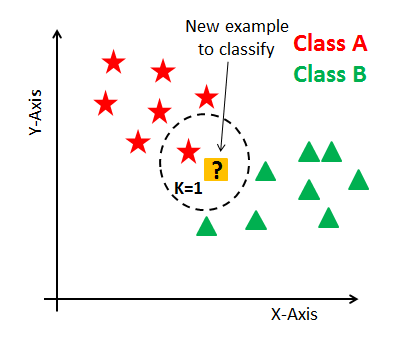
\includegraphics[scale=0.6]{pages/Chapter2/Chapter 2 images/knn.png}
    \caption{Classification of a test point with kNN. \textit{Sourced from} \cite{chauhan_2019}.}
    \label{fig_knn}
\end{figure}
 
\subsubsection{XGBoost}
XGBoost which is also known as ``\textit{e\textbf{X}treme \textbf{G}radient \textbf{B}oosting}" is a type of supervised learning algorithm used in machine learning. It is the implementation of gradient boosting machines or boosted decision trees where it heavily focuses on optimization and scalability. The XGBoost algorithm is used to solve regression and classification problems. This algorithm uses the concept of decision trees where features are split further into intervals to classify data in the form of nodes and branches.

The hyperparameters of this algorithm includes the number of classes involved, learning rate, gamma and subsamples. The number of classes represents the number of target variables available in the data provided. The learning rate prevents the overfitting of data where the trained model is only able to predict values that exist in the the training set.
Overfitting implies that the model trains by including noise or existing anomalies in the provided dataset. The subsample and gamma hyperparameter shares the similar concept as well to prevent overfitting of the machine learning model. 

\subsection{Machine Learning Model Performance Evaluation}
The final performance of the machine learning model will be evaluated using the split test data. Metrics such as the confusion matrix can be used to measure the performance of the trained model. Several parameters can be obtained from the confusion matrix such as accuracy, sensitivity, precision and specificity. The confusion matrix is a N x N matrix which shows the number of classified and misclassified data for N classes of data. An example of a confusion matrix can be shown in \ref{fig_cf}.

\begin{figure} [ht]
    \centering
    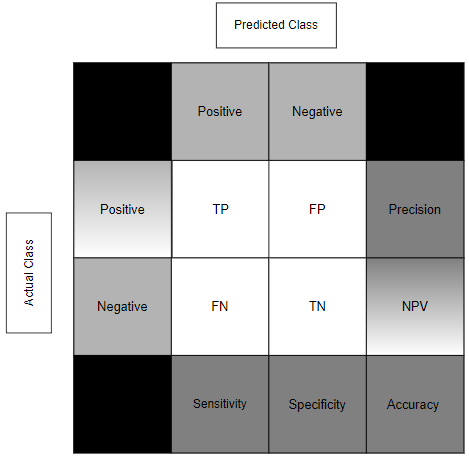
\includegraphics[scale=1.0]{pages/Chapter2/Chapter 2 images/Confusion matrix.PNG}
    \caption{Confusion matrix.}
    \label{fig_cf}
\end{figure}

From fig. \ref{fig_cf}, TP, FP, FN and TN represents true positive, false positve, false negative and true negative respectively. True positive and true negative represent data predicted correctly with the actual class while false positive and false negative are misclassified data predicted under the in incorrect class.
The accuracy of the model which represents the data are classified under the correct class can be evaluated with \ref{eq:3}.
\begin{equation}
    Accuracy(\%) = \frac{TP + TN}{TP+TN+FN+FP} X100\% 
    \label{eq:3}
\end{equation}

Specificity measures the frequency of data predicted correctly under the negative actual class as shown in \ref{eq:4}. 
\begin{equation}
    Specificity(\%) = \frac{TN}{FP+TN} X100\% 
    \label{eq:4}
\end{equation}

Sensitivity shows the data correctly under the positive class and can be computed  with \ref{eq:5}.
\begin{equation}
    Sensitivity(\%) = \frac{TP}{TP+FN} X100\% 
    \label{eq:5}
\end{equation}

Thus, the confusion matrix is one of the several useful metrics to determine the performance of a machine learning model before getting it ready for deployment.





%     1. Introduction including the following points: (i) what is the required product and how it will be applied. The name of the organisation of the external partner and names of the contact(s) (ii) why the product should be created (Societal, environmental, economic (competing technologies and advantages over these?) (iii) the main field, technology area of your external partner and the rational as to why the external partner wishes for the product to be created and who will exploit it (non-expert/expert, other engineer/research area) (iv) Clearly identify whether the output required by the external partner is a 'proof of concept', demonstrator or application of an existing technology (for a trade show for instance), a prototype or an elaboration or add-on of/intergration with/ superseeds an existing system.
